% \section{The Unified Modeling Language and the Eclipse Modeling Framework} 
UML provides a range of languages for modeling purposes.
We need languages to describe metamodels and models.
For models, UML provides Object Diagrams, and for metamodels, Class Diagrams and the Object Constraint Language.
Additionally, we will use C-like syntax for Class specifications.

\subsection{Meta-Object Facility}
The Unified Modeling languguage is build ontop of the Meta-Object Facility standard.
Formally: the UML metamodel conforms to MOF meta-metamodel.
MOF provides a meta-metamodel similar to that presented in the previous section.

The MOF standard also describes a four layer model hirearchy illustraiting its application.
The MOF meta-metamodel exists as the top layer of abstraction in the MOF architecture, the M3 layer.
The MOF architecture has three lower layers of abstraction, the lowest being that of the system under study, the M0 layer.
UML exists at the M2 layer, and the M1 layer contains the UML conforming models and metamodels created by the user to represent the system under study.

\begin{figure}[h]
    \centering
    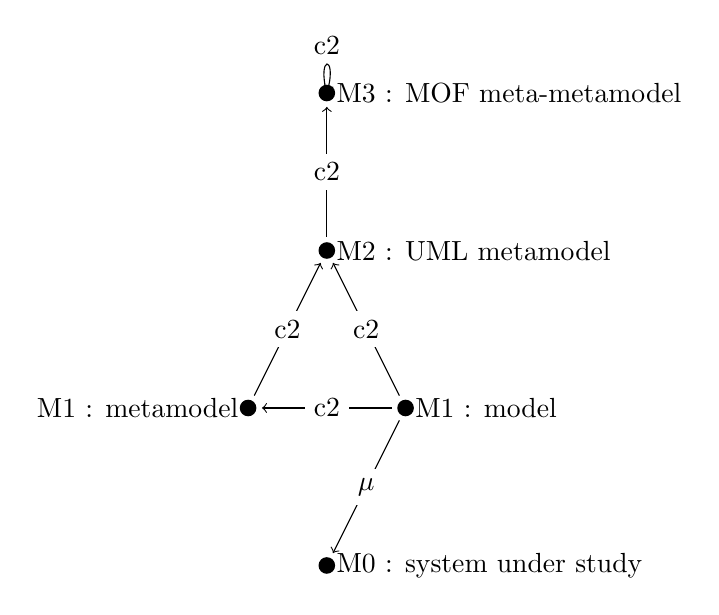
\begin{tikzpicture}
        \coordinate [label=0:{M0 : system under study}] (M0) at (0,0);
        \coordinate [label=180:{M1 : metamodel}]  (M1) at (-1,2);
        \coordinate [label=0:{M1 : model}]  (M12) at (1,2);
        \coordinate [label=0:{M2 : UML metamodel}]  (M2) at (0,4);
        \coordinate [label=0:{M3 : MOF meta-metamodel}]  (M3) at (0,6);

        % \coordinate [label=0:{XMI : model}]  (E1) at (6,2);
        % \coordinate [label=0:{Ecore : metamodel}]  (E2) at (6,4);
        % \coordinate [label=0:{Ecore : meta-metamodel}]  (E3) at (6,6);
      
          \fill (M0) circle (3pt);
          \fill (M1) circle (3pt);
          \fill (M12) circle (3pt);
          \fill (M2) circle (3pt);
          \fill (M3) circle (3pt);

        %   \fill (E1) circle (3pt);
        %   \fill (E2) circle (3pt);
        %   \fill (E3) circle (3pt);
          
        \draw[->, shorten <= 5pt, shorten >= 5pt,] (M12) -- (M0) node [midway,fill=white] {$\mu$};
        \draw[->, shorten <= 5pt, shorten >= 5pt,] (M12) -- (M2) node [midway,fill=white] {c2};
        \draw[->, shorten <= 5pt, shorten >= 5pt,] (M12) -- (M1) node [midway,fill=white] {c2};
        \draw[->, shorten <= 5pt, shorten >= 5pt,] (M1) -- (M2) node [midway,fill=white] {c2};
        \draw[->, shorten <= 5pt, shorten >= 5pt,] (M2) -- (M3) node [midway,fill=white] {c2};

        % \draw[->, shorten <= 5pt, shorten >= 5pt,] (E1) -- (E2) node [midway,fill=white] {conforms-to};
        % \draw[->, shorten <= 5pt, shorten >= 5pt,] (E2) -- (E3) node [midway,fill=white] {conforms-to};
        % \draw[->, shorten <= 5pt, shorten >= 5pt,] (M3) -- (M3) node [midway,fill=white] {conforms-to};
        % \draw (1pt,\y cm) -- (-1pt,\y cm) node[anchor=east] {$\mathbf{\y}$};
        \path[->] (M3) edge [loop above] node {c2} ();
    \end{tikzpicture}
    \caption{Meta-Object Facility model hierarchy}
\end{figure}

\subsection{Class Diagrams}
Class Diagrams identify concepts and their properties.
In a family tree for instance, the core concept is Person, with attributes such as age and references such as parent (or its opposite, child) to express relationships between people. 
%a relation of the person such as \emph{parent} or it's opposite \emph{child} would be a reference type property, an example attribute would be age.

\begin{figure}[!ht]
    \centering
    \includegraphics[trim={0 0 0 0},width=1\linewidth]{Articles/ICTAI2025/figures/metamodel.pdf}
    \caption{UML Class Diagram as Metamodel}
    \label{fig:metamodel}
\end{figure}
In this figure we see a rectangle with a title, which represents a class.
In the rectangle beneath the title, we find a list of attribute properties.
From the rectangle to itself, we see an arrow representing the reference property.
Here we present a generic metamodel.
It describes a class named \inlineocl{Object}, which has two properties: 
\inlineocl{attribute}: a collection of integers, with at least one and at most $m$ elements, \inlineocl{reference}: a collection of up to $n$ references to other \inlineocl{Object} instances.
%\inlineocl{reference} a collection of up to $n$ objects and \inlineocl{attribute} a collection of at least one and at most $m$ integers.
These illustrate the two main types of properties in object-oriented modeling:
Attributes, which store intrinsic data values (e.g., numbers or strings),
References, which define relationships between objects in the model.

%These are illustrative of the two types of object property : references and attributes.
%References describe the relations across a graph of objects, whereas attributes colour the graph nodes.
\subsubsection{UML Collection Types}
UML allows properties to be collections, and distinguishes four standard collection types, based on two dimensions: order and uniqueness.
%Properties are generally collections of elements, and UML distinguishes between 4 concrete collection types: \inlineocl{Sequence}, \inlineocl{Bag}, \inlineocl{OrderedSet} and \inlineocl{Set}.
%hese collection types exist at the intersection between two qualities: orderedness and uniqueness.
\begin{itemize}
    \item \inlineocl{Sequence}: ordered, allows duplicates -- e,g., [2,3,1,1],
   % has ordered non-unique elements:\\ ~[2,3,1,1] has information about order such as \emph{3 before 1}, and repeated values.
    \item \inlineocl{Bag}: unordered, allows duplicates -- e.g., [1,1,2,3], 
    %has non-unique non-ordered elements:\\~[1,1,2,3] has repeated values but we've lost the order.
    \item \inlineocl{Set}: unordered, unique elements only -- e.g., [1,2,3], 
    %has unique non-ordered elements:\\~[1,2,3] has no order and no repeated values.
    \item \inlineocl{OrderedSet}:  ordered, unique elements -- e.g., [2,3,1]. 
    %has order across unique elements:\\ ~[2,3,1] has order but no repeating values.
\end{itemize}
\textcolor{black}{An important note is that \emph{ordered} doesn't pertain to the values.
In [2,3,1,1]: 2 is the \emph{first} value, and 1 is the \emph{last} value. 
}
The intended collection type can be indicated in the class diagram using annotations such as \inlineocl{ordered}, \inlineocl{unique}, or \inlineocl{seq} (for sequences).
%To indicate the collection type of a property in the class diagram, the properties can be annotated with the words \inlineocl{ordered}, \inlineocl{unordered}, \inlineocl{unique}, \inlineocl{ordered} or \inlineocl{seq} (for sequences).
% In modeling tools like the Eclipse Modeling Framework (EMF), class diagrams can be used to automatically generate code. For example, the diagram in Figure \ref{fig:metamodel} could yield the following class definition in an object-oriented programming language:
% %Within a framework such as the Eclipse Modeling Framework, these kinds of diagram can be used to generate code. For instance, from Figure \ref{fig:metamodel} we could generate a class description in an object-oriented programming language:
% \begin{lstlisting}
% class Object {  attribute : int[1..3]
%                 reference : Object[0..2]}
% \end{lstlisting}
% Code generation includes not only class definitions but also methods (getters/setters) and factory mechanisms for instantiating objects and populating models from data sources (e.g., EMF's XMI serialization).
%and generate getters, setters and factories to build these objects when loading data from an EMF model.

% \subsection{Object Diagrams}
% \smallskip
% \noindent \label{ssec:ctxt_id}
\subsubsection{UML Reference Types}
UML also gives us different kinds of relations between objects, notably containment relations and and opposite relations.

\noindent \textbf{Opposite} 
The opposite of \textit{child-of} for instance, is \textit{parent-of}.
Sometimes references may need to be one-way for encapsulation.

\noindent \textbf{Containment} means that the \textit{contained} object is only related to one \textit{container} object through this instance of the relation.



\subsection{Object Diagrams}
% Object diagrams 
describe instances of the classes defined in a class diagram.
%Object (or instance) diagrams show the data, as instances of the concepts described in a class diagram.
For example, Figure~\ref{fig:model} shows an instance conforming to the class diagram in Figure~\ref{fig:metamodel}. It includes three objects, each identified by a unique ID (e.g., \inlineocl{o1}, \inlineocl{o2}, \inlineocl{o3}). For instance, object \inlineocl{o1} has as attribute a collection of 3 integers and is connected to other objects (e.g., \inlineocl{o2} and \inlineocl{o3}).
% Similarly to class diagrams, EMF also supports the use of object diagrams to visually manipulate data instances. 

% which are the maximums allowed by our choice of $n=2$ and $m=3$.

% A family tree is an example of an instance diagram;
% previously, we declared what concepts make up a family tree, but an actual family tree needs instances of related people.
\begin{figure}[!ht]
    \centering
    \includegraphics[trim={0 0 0 0},width=1\linewidth]{Articles/ICTAI2025/figures/model.pdf}
    \caption{UML Instance Diagram as Model}
    \label{fig:model}
\end{figure}
This diagram is also built from rectangles and lines connecting them.
Here each rectangle represents an object, and the title area is used to give the \texttt{:Type} and optionally a name.
Below the title area, we again use the rectangle to list the attributes and the information associated.
The arrows between the rectangles represent instances of the references between objects.
In Figure \ref{fig:model} we see a model which conforms to the metamodel from Figure \ref{fig:metamodel}, for which we chose $n=2$ and $m=3$. This here shows objects of the type described by the class, and the values assigned to their properties.
% This instance will serve to illustrate the result of queries and the operations upon them.
In this model, \inlineocl{o2 : Object} is an instance of the \inlineocl{Object} class named \inlineocl{o2}, as attribute it has a collection of integers with a single value: 1000.
The object \inlineocl{o1} has as attribute a collection of 3 integers and is connected to both other objects, which are the maximums allowed by our choice of $n=2$ and $m=3$.

% These instances can be serialized using the XML Metadata Interchange (XMI) format.
%Similarly to class diagrams, EMF allows us to use object diagrams to manipulate instances of data visually.
%Such an instance would be serialized in the XML Metadate Interchange format.